% Referências em
%% http://www.abntex.net.br/
% ------------------------------------------------------------------------
% ------------------------------------------------------------------------
% Template adaptado por Armando Leopoldo Keller - Unisinos
% ------------------------------------------------------------------------
% ------------------------------------------------------------------------



\documentclass[
	% -- opções da classe memoir --
	12pt,				% tamanho da fonte
	%openright,			% capítulos começam em pág ímpar (insere página vazia caso preciso)
	oneside,
	%twoside,			% para impressão em recto e verso. Oposto a oneside
	a4paper,			% tamanho do papel. 
	% -- opções da classe abntex2 --
	chapter=TITLE,		% títulos de capítulos convertidos em letras maiúsculas
	section=TITLE,		% títulos de seções convertidos em letras maiúsculas
	%subsection=TITLE,	% títulos de subseções convertidos em letras maiúsculas
	%subsubsection=TITLE,% títulos de subsubseções convertidos em letras maiúsculas
	% -- opções do pacote babel --
	english,			% idioma adicional para hifenização
	french,				% idioma adicional para hifenização
	spanish,			% idioma adicional para hifenização
	brazil				% o último idioma é o principal do documento
	]{abntex2}

\usepackage{unisinos} % Necessário para customização para padrão da universidade

% ---
% Pacotes básicos 
% ---
\usepackage[T1]{fontenc}		% Selecao de codigos de fonte.
\usepackage[utf8]{inputenc}		% Codificacao do documento (conversão automática dos acentos)
\usepackage{indentfirst}		% Indenta o primeiro parágrafo de cada seção.
\usepackage{color}				% Controle das cores
\usepackage{graphicx}			% Inclusão de gráficos
\usepackage{microtype} 			% para melhorias de justificação
\usepackage[table,xcdraw]{xcolor} %para cores nas tabelas
\usepackage{verbatim}           %para comentários
%\usepackage{float}
\usepackage{placeins}
\usepackage{booktabs}
\usepackage{pdfpages}
% ---
		
% ---
% Pacotes adicionais: Insira aqui os pacotes customizados para todo o documento
% ---
\usepackage{lipsum}				% para geração de dummy text
% ---

\usepackage{helvet}                         % Configuração da fonte padronizada no documento
\renewcommand{\familydefault}{\sfdefault}

% ---
% Pacotes de citações
% ---
\usepackage[brazilian,hyperpageref]{backref}	 % Paginas com as citações na bibl
\usepackage[alf]{abntex2cite}	% Citações padrão ABNT

% --- 
% CONFIGURAÇÕES DE PACOTES
% --- 

% ---
% Configurações do pacote backref
% Usado sem a opção hyperpageref de backref
\renewcommand{\backrefpagesname}{Citado na(s) página(s):~}
% Texto padrão antes do número das páginas
\renewcommand{\backref}{}
% Define os textos da citação
\renewcommand*{\backrefalt}[4]{
	\ifcase #1 %
		Nenhuma citação no texto.%
	\or
		Citado na página #2.%
	\else
		Citado #1 vezes nas páginas #2.%
	\fi}%
% ---


% ||||||||||||||||||||||||||||||||||||||||||||||
% Informações de dados para CAPA e FOLHA DE ROSTO
% ||||||||||||||||||||||||||||||||||||||||||||||
\newcommand{\varCurso}{Engenharia Eletrônica }
\titulo{ACOMPANHAMENTO DIGITAL DA LOGÍSTICA DE PRODUTOS PERECÍVEIS}
\autor{HUMBERTO CORRÊA KRAMM}
\local{São Leopoldo, RS}
\data{2022}
\orientador{Prof. Dr. Sandro Binsfeld Ferreira} 
% ---
% Informações de dados para CAPA e FOLHA DE ROSTO
% ---

%\coorientador{Equipe \abnTeX}
\instituicao{%
  UNIVERSIDADE DO VALE DO RIO DOS SINOS -- UNISINOS
  \par
  UNIDADE ACADÊMICA DE GRADUAÇÃO
  \par
  CURSO DE \MakeUppercase{\varCurso}}
\tipotrabalho{Monografia (graduação)}
% O preambulo deve conter o tipo do trabalho, o objetivo, 
% o nome da instituição e a área de concentração 
\preambulo{Trabalho de Conclusão de curso apresentado como requisito parcial para obtenção do título de Bacharel em \varCurso, pelo curso de \varCurso da Universidade do Vale do Rio dos Sinos (UNISINOS).}
% ---


% ---
% Configurações de aparência do PDF final

% alterando o aspecto da cor azul
\definecolor{blue}{RGB}{41,5,195}
%\definecolor{blue}{RGB}{0,0,0}



% informações do PDF
\makeatletter
\hypersetup{
     	%pagebackref=true,
		pdftitle={\@title}, 
		pdfauthor={\@author},
    	pdfsubject={\imprimirpreambulo},
	    pdfcreator={LaTeX with abnTeX2},
		pdfkeywords={abnt}{latex}{abntex}{abntex2}{trabalho acadêmico}, 
		colorlinks=false,%true,       		% false: boxed links; true: colored links
    	linkcolor=blue,          	% color of internal links
    	citecolor=blue,        		% color of links to bibliography
    	filecolor=magenta,      		% color of file links
		urlcolor=blue,
		anchorcolor =red,
		bookmarksdepth=4
}

\makeatother
% --- 

% ---
% Posiciona figuras e tabelas no topo da página quando adicionadas sozinhas
% em um página em branco. Ver https://github.com/abntex/abntex2/issues/170
\makeatletter
\setlength{\@fptop}{5pt} % Set distance from top of page to first float
\makeatother
% ---

% ---
% Possibilita criação de Quadros e Lista de quadros.
% Ver https://github.com/abntex/abntex2/issues/176
%
\newcommand{\quadroname}{Quadro}
\newcommand{\listofquadrosname}{Lista de quadros}

\newfloat[chapter]{quadro}{loq}{\quadroname}
\newlistof{listofquadros}{loq}{\listofquadrosname}
\newlistentry{quadro}{loq}{0}

% configurações para atender às regras da ABNT
\setfloatadjustment{quadro}{\centering}
\counterwithout{quadro}{chapter}
\renewcommand{\cftquadroname}{\quadroname\space} 
\renewcommand*{\cftquadroaftersnum}{\hfill--\hfill}

\setfloatlocations{quadro}{hbtp} % Ver https://github.com/abntex/abntex2/issues/176
% ---

% --- 
% Espaçamentos entre linhas e parágrafos 
% --- 

% O tamanho do parágrafo é dado por:
\setlength{\parindent}{1.3cm}

% Controle do espaçamento entre um parágrafo e outro:
\setlength{\parskip}{0.2cm}  % tente também \onelineskip

% ---
% compila o indice
% ---
\makeindex
% ---

% ----
% Início do documento
% ----
\begin{document}

% Seleciona o idioma do documento (conforme pacotes do babel)
%\selectlanguage{english}
\selectlanguage{brazil}

% Retira espaço extra obsoleto entre as frases.
\frenchspacing 

% ----------------------------------------------------------
% ELEMENTOS PRÉ-TEXTUAIS
% ----------------------------------------------------------
% \pretextual

% ---
% Capa
% ---
\imprimircapa
% ---

% ---
% Folha de rosto
% (o * indica que haverá a ficha bibliográfica)
% ---
%\imprimirfolhaderosto*
\imprimirfolhaderosto
% ---



% ---
% Agradecimentos
% ---
\begin{agradecimentos}
Aos seres humanos...... 

\end{agradecimentos}
% ---

% ---
% Epígrafe
% ---

\begin{comment}
Epígrafe (Não se escreve a palavra epígrafe). Elemento opcional. 
A epígrafe deve ser colocada após o agradecimento; trata-se de uma citação, seguida de indicação de autoria, relacionada à matéria tratada no corpo do trabalho. Deve ser “[...] elaborada conforme a NBR 10520 [...]. Podem também constar epígrafes nas folhas ou páginas de abertura das seções primárias” (ABNT, 2002, p. 7). 
A fonte da epígrafe deve sempre ser mencionada nas referências. 

Citação direta até 3 linhas deve estar entre aspas e em parágrafo normal (vá até a janela de Estilo - selecione - Parágrafo), se tiver mais de 3 linhas, deve ser recuada 4 cm da margem esquerda, com fonte menor que 12 e espaçamento entre linhas simples 
\end{comment}

\begin{epigrafe}
    \vspace*{\fill}
	\begin{flushright}
		\textit{“42 is the Answer to the Ultimate Question of Life, the Universe, and Everything.”  \\
        \citeonline{adams2007hitchhiker}
}
	\end{flushright}
\end{epigrafe}
% ---

% ---
% RESUMOS
% ---

% resumo em português
\setlength{\absparsep}{18pt} % ajusta o espaçamento dos parágrafos do resumo
\begin{resumo}
    A crescente demanda de dispositivos iot vem acompanhada de uma carência tecnológica por baterias eficientes para garantir a flexibilidade dos sistemas que necessitam estar desconectados de cabos. Neste trabalho, será explorado \textit{Energy Harvesting} como técnica de obtenção de energia para dispositivos iot que tem como princípio a utilização do meio para obtê-las. Esta técnica tem como objetivo aproveitar a energias do meio em que o dispositivo se encontra como a solar, cinética, térmica entre outras. Este trabalho se propõe a coletar a energia das emissões de rádio frequência do meio ao longo de um tempo para uma transmissão em um momento oportuno. Desta forma, os paradigmas que se apresentam giram em torno de uma comunicação de baixo consumo e um gerenciamento eficiente para armazenagem desta potência. Neste cenário, parte-se de alternativas como o HT32SX que foi construído para atender demandas de extremamente baixo consumo e rádio integrado que pode ser adaptado para diversas aplicações de transmissão de dados também com pouco consumo. Com isso, espera-se projetar um dispositivo iot com uma linha de comunicação capaz de ser independente de cabos ou baterias.

 \textbf{Palavras-chave}: Energy Harvesting, low power, iot, LP Wan.
\end{resumo}

% resumo em inglês
\begin{resumo}[Abstract]
 \begin{otherlanguage*}{english}
The growing demand for iot devices is accompanied by a technological need for efficient batteries to ensure the flexibility of systems that need to be disconnected from cables. In this work, Energy Harvesting will be approached as a technique for obtaining energy for iot devices that has as its principle the use of the medium to obtain them. This technique aims to take advantage of the energies of the environment in which the device is located, such as solar, kinetic, thermal, among others. This work proposes to collect the energy of radio frequency emissions from the medium over a period of time for a transmission at an opportune moment. In this way, the paradigms that are presented revolve around a low consumption communication and an efficient management for the storage of this power. In this scenario, we start with alternatives such as the HT32SX, which was built to meet the demands of extremely low consumption and an integrated radio that can be adapted for various data transmission applications also with little consumption. With this, it is expected to design an iot device with a communication line capable of being independent of cables or batteries.

   \vspace{\onelineskip}
 
   \noindent 
   \textbf{Keywords}: Energy Harvesting, low power, iot, LP Wan.
 \end{otherlanguage*}
\end{resumo}


% ---
% inserir lista de ilustrações
% ---
\pdfbookmark[0]{\listfigurename}{lof}
\listoffigures*
\cleardoublepage
% ---

% ---
% inserir lista de quadros
% ---
\pdfbookmark[0]{\listofquadrosname}{loq}
\listofquadros*
\cleardoublepage
% ---

% ---
% inserir lista de tabelas
% ---
\pdfbookmark[0]{\listtablename}{lot}
\listoftables*
\cleardoublepage
% ---

% ---
% inserir lista de abreviaturas e siglas
% ---
\begin{siglas}
    \item[AD] \textit{Analógico-Digital}
    \item[Anatel]   \textit{Agência Nacional de Telecomunicações}
    \item[CI]   \textit{Circuito integrado}
    \item[CMOS] \textit{Complementary metal–oxide–semiconductor} (metal-óxido-semicondutor de simetria complementar)
    \item[DBPSK]    \textit{differential binary phase shift keying} (Modulação por chaveamento de deslocamento de fase binária diferencial)
    \item[DC]  \textit{Direct Current} (Corrente contínua)
    \item[FLV] \textit{Frutas, Verduras e Legumes}
    \item[FSK] \textit{Frequency Shifting Keying} (Modulação por chaveamento de frequência)
    \item[GPIO]     \textit{General Purpose Input/Output} (Entradas e Saídas de uso Geral)
    \item[EH]   \textit{Energy Harvesting} (Coleta de Energia) 
    \item[I2C]  \textit{Inter-Integrated Circuit} (Comunicação Entre circuitos Integrados)
    \item[IOT]  \textit{Internet of Things} (Internet das coisas)
    \item[ISM]  \textit{industrial, scientific and medical}(Indústria, Ciência e Medicina)
    \item[LoRa] \textit{Long Range} (Longo alcance)
    \item[LPWAN] \textit{Low-power wide-area network} (Redes de longa distância de baixa potência)
    \item[M2M] \textit{machine-to-machine} (Máquina à máquina) 
    \item [MLP] \textit{Multilayer Perceptron} (Perceptron multicamadas)
    \item[RF]  \textit{Rádio Frequência}
    \item[RTC]  \textit{Real-time clock} (Relógio de tempo real)
    \item[UNISINOS]  \textit{Universidade do Vale do Rio dos Sinos}

\end{siglas}
% ---

% ---
% inserir lista de símbolos
% ---
\begin{simbolos}
  \item[$t$] Tempo
  \item[$dt$] Diferencial de tempo
  \item[$V_a$] Tensão da fonte
\end{simbolos}
% ---

% ---
% inserir o sumario
% ---
\pdfbookmark[0]{\contentsname}{toc}
\tableofcontents*
\cleardoublepage
% ---


% ----------------------------------------------------------
% ELEMENTOS TEXTUAIS
% ----------------------------------------------------------
\textual

% ----------------------------------------------
\chapter{INTRODUÇÃO}\label{cap:introducao}
% ----------------------------------------------
A base para o desenvolvimento de um sistema de monitoramento digital capaz de acompanhar produtos perecíveis, passa por um entendimento de todos os elos envolvidos. Dentre eles a dinâmica entre a temperatura e o crescimentos de vida microbiana (Listeria) bem como a logística nacional para esse tipo de alimento. Além disso, deve-se considerar também as limitações técnicas para o desenvolvimento de dispositivos IoT capazes de obter dados críticos de todo o processo.
% ----------------------------------------------
\section{TEMA} 
% ----------------------------------------------
Neste trabalho pretende-se propor um dispositivo capaz acompanhar o deslocamento de um determinado alimento perecível. Para isso, esse dispositivo, necessita possuir alguns requisitos como:
\begin{itemize}
    \item Baixo valor agregado, uma vez que precisa ser empregado em caixas de transporte de alimentos;
    \item Ocupar a menor área possível;
    \item Operar sem a necessidade trocas de pilhas ou recarregamento de baterias;
\end{itemize}
% ----------------------------------------------
\section{DELIMITAÇÃO DO TEMA} 
% ----------------------------------------------
Neste trabalho pretende-se propor um dispositivo capaz acompanhar o deslocamento de um determinado alimento perecível. Para isso, esse dispositivo, necessita possuir alguns requisitos como:
\begin{itemize}
    \item Baixo valor agregado, uma vez que precisa ser empregado em caixas de transporte de alimentos;
    \item Ocupar a menor área possível;
    \item Operar sem a necessidade trocas de pilhas ou recarregamento de baterias;
\end{itemize}

A definição destes requisitos, passa também por um entendimento das condições de operação e ambiente a que esse sistema está submetido, bem como os agentes envolvidos para um correto entendimento do cenário completo.
% ----------------------------------------------
\section{PROBLEMA}
% ----------------------------------------------



% ----------------------------------------------
\section{OBJETIVOS}
% ----------------------------------------------
%%%%%%%%%%%%%%%%%%%%%%%%%%%%%%%%%%%%%%%%%%%%%%%%%%%%%%%%%%%%%%%%%%%%%%
\subsection{Produtos perecíveis}
%%%%%%%%%%%%%%%%%%%%%%%%%%%%%%%%%%%%%%%%%%%%%%%%%%%%%%%%%%%%%%%%%%%%%%
Denominam-se alimentos perecíveis aqueles que possuem uma quantidade significativa de água. Isso os torna vulneráveis a proliferação de vida microbiana que é a principal responsável pela decomposição destes alimentos. Para se manterem conservados, estes alimentos necessitam manter-se refrigerados.
Alimentos perecíveis estão presentes no dia a dia das populações no mundo inteiro, pois muitos deles são a base de uma alimentação saudável devido a pouca exposição a conservantes ou processos industriais que embora eliminem as suas bactérias, acabam por eliminar também os seus nutrientes.
Com o objetivo de mapear a composição dos principais alimentos consumidos no Brasil, a \citeonline{Anvisa2011} desenvolveu o projeto TACO (Tabela Brasileira de Composição de Alimentos). A partir desta, obteve-se um detalhamento da tabela nutricional e demais dados dos alimentos que compõe o dia a dia dos brasileiros.

Com base nisso, apresenta-se um problema relacionado a distribuição destes alimentos ao longo de um país como o Brasil que possui dimensões continentais e alguns alimentos são produzidos apenas em certas regiões.
Com o objetivo de predizer o impacto do aumento de listeria \citeonline{monica} apresenta um algorítimo baseado em redes neurais artificiais \textit{Multilayer Perceptron} (MLP) em função dos impactos atmosféricos a que esses alimentos são submetidos. A capacidade de prever a vida útil destes alimentos a partir de fatores ambientais pode ser decisivo para a escolha do meio de transporte do mesmo e para o aumento das exigências de qualidade que redes atacadistas impõe no ato de revenda dos mesmos.

%%%%%%%%%%%%%%%%%%%%%%%%%%%%%%%%%%%%%%%%%%%%%%%%%%%%%%%%%%%%%%%%%%%%%%
\subsection{Logística}
%%%%%%%%%%%%%%%%%%%%%%%%%%%%%%%%%%%%%%%%%%%%%%%%%%%%%%%%%%%%%%%%%%%%%%
Dentro de uma cadeia de distribuição de alimentos, existe uma série de desafios logísticos envolvidos no processo e todos esses processos são responsáveis por um grau de depreciação na vida útil de alimentos como frutas, verduras e legumes (FLV). Analisar essa cadeia é essencial para compreender que quanto mais elementos envolvidos, como intermediários, maior as chances de se perder a rastreabilidade e a qualidade dos FLV.
Os autores \citeonline{Aliotte2022} detalham que os fatores mais importantes a serem observados no processo de distribuição são:
\begin{itemize}
    \item Tipo de transporte
    \item Agente responsável pelo transporte
    \item Rastreabilidade
    \item Acondicionamento em câmara fria
    \item Tipos de embalagem
    \item Troca de embalagem
    \item Manipulação da carga
\end{itemize}

Dentre estes, cabe destaque para o tipo de transporte, que pode ser do tipo caminhão baú frigorificado que pode oferecer temperaturas abaixo de $0^oC$; caminhão baú refrigerado que pode manter temperaturas entre $0^oC$ e $12^oC$; caminhão graneleiro que possui apenas proteção com lona para orvalho, sol e chuva e não possui controle de refrigeração; caminhão baú sem refrigeração que se assemelha ao graneleiro; além do caminhão com carroceria aberta. Na figura~\ref{fig:transporte} é possível ver a distribuição de uso destes caminhões para alguns tipos de cargas.

\begin{figure}
  \caption{Transporte por tipo de carroceria.}
  \begin{center}
      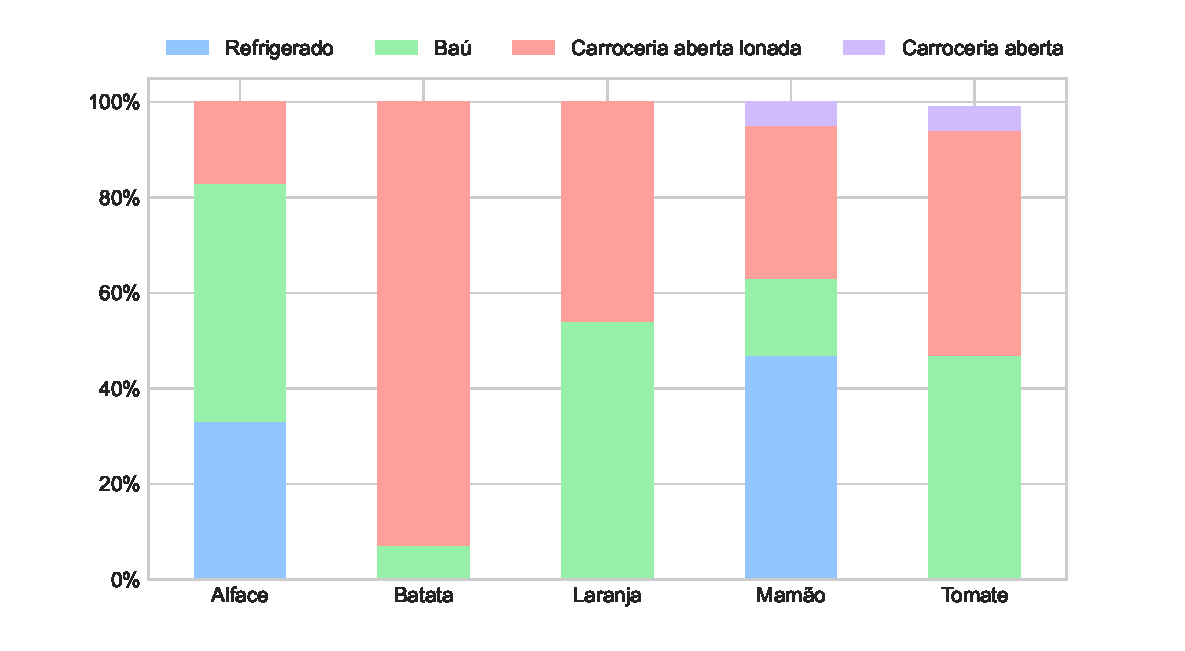
\includegraphics[trim={0 1.2cm 0 0.5cm },scale=0.6]{img/transporte.pdf}
  \end{center}
  \fonte{Elaborado pelo autor com base em~\cite{Aliotte2022} }
  \label{fig:transporte}
\end{figure}

Uma vez introduzidas as diferentes formas de transporte \citeonline{Aliotte2022} discorrem sobre os agentes responsáveis pelo transporte e suas particularidades. Fatores como distância a ser percorrida e a terceirização do transportes são efetivamente relevantes, impactando diretamente na qualidade dos FLV.

Ao tratar da rastreabilidade e acondicionamento em câmara fria, \citeonline{Aliotte2022} apontam uma demanda do mercado por qualidade. Fica evidente que investimentos nessas áreas possuem um apelo não só para atender consumidores exigentes como normas sanitárias.

Já os três últimos tópicos: tipos de embalagem, troca de embalagem e manipulação da carga, dizem respeito aos impactos da embalagem tanto ao condicionamento como ao desgaste ocasionados no processo de alocação.

``Para que o produto chegue ao destino em boas condições, é necessário que ocorra o mínimo de manuseio, que sejam cumpridas as regras sanitárias nas operações de carga e descarga, além do uso de tecnologias que reduzam a manipulação por ação humana.'' \cite[p.~16]{Aliotte2022}





%%%%%%%%%%%%%%%%%%%%%%%%%%%%%%%%%%%%%%%%%%%%%%%%%%%%%%%%%%%%%%%%%%%%%%
\subsection{IoT}
%%%%%%%%%%%%%%%%%%%%%%%%%%%%%%%%%%%%%%%%%%%%%%%%%%%%%%%%%%%%%%%%%%%%%%
O termo \textit{Internet of Things} (IOT), traduzido livremente para ``Internet das Coisas'', popularizou-se nos últimos anos devido aos avanços tecnológicos em termos de miniaturização de circuitos eletrônicos. Graças a esses avanços, um mundo de opções se abriu para resolver problemas que antes eram impossíveis como o controle de iluminação artificial em uma horta apresentado por \citeonline{9268238} que controla um sistema de espelhos para garantir um adequado fornecimento de luz, além de coletar informações disponibilizando-as em uma plataforma web.

Dispositivos IOT tem como princípio básico o acesso direto a internet, seja para apenas enviar informações, apenas receber ou ambos. A principal vantagem desses sistemas se dá em função da possibilidade de externar o processamento, garantindo assim um requisito de hardware mínimo local, deixando tarefas complexas para a rede externa (Nuvem).  

A popularização dos sistemas IOT se dá de forma tão rápida que até mesmo problemas decorrentes da sincronização de dispositivos passam a ser tratados com soluções como a apresentada por \citeonline{7924944}. Já aplicações que perdem a adesão são rapidamente descontinuadas como a solução da empresa Amazon para comprar sabão de roupas com um botão instalado na maquina de lavar\citeonline{amazon} mostrado na figura~\ref{fig:amazon}.

\begin{figure}
  \caption{Amazon Dash Button.}
  \begin{center}
      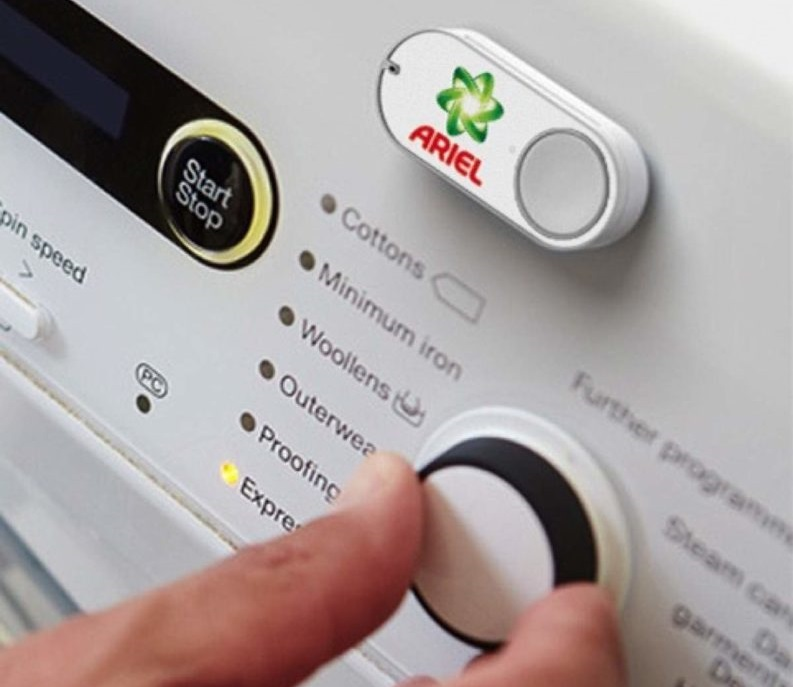
\includegraphics[scale=0.6]{img/Amazon-Dash-Button.png}
  \end{center}
  \fonte{\citeonline{amazondash}}
  \label{fig:amazon}
\end{figure}

Segundo \citeonline{8648462}, os principais desafios para empregabilidade de sistemas IOT são a extrema heterogeneidade que diz respeito aos diferente tipos de dispositivos e protocolos envolvidos, a dinâmica imprevisível que diz respeito aos ambientes distintos e obstáculos físicos além da escalabilidade no núcleo que trata dos problemas que envolvem o acesso de vários dispositivos a uma mesma nuvem. Este último, se apresenta como grande relevância para os próximos anos, pois o aumento da quantidade de ``coisas'' ligadas a internet tendem a crescer em demasia.

%%%%%%%%%%%%%%%%%%%%%%%%%%%%%%%%%%%%%%%%%%%%%%%%%%%%%%%%%%%%%%%%%%%%%%

%%%%%%%%%%%%%%%%%%%%%%%%%%%%%%%%%%%%%%%%%%%%%%%%%%%%%%%%%%%%%%%%%%%%%%










\chapter{Fundamentação teórica}
%\section{Revisão bibliográfica}
Neste capítulo analisou-se a bibliografia existe e executou-se uma revisão em trabalhos correlatos. Nela pesquisou-se sobre arquiteturas de rede disponíveis para utilização durante comunicações de dispositivos IoT, bem como técnicas para aproveitamento de energia disponíveis no ambiente.

%%%%%%%%%%%%%%%%%%%%%%%%%%%%%%%%%%%%%%%%%%%%%%%%%%%%%%%%%%%%%%%%%%%%%%
\section{LPWAN} %ch 1303
%%%%%%%%%%%%%%%%%%%%%%%%%%%%%%%%%%%%%%%%%%%%%%%%%%%%%%%%%%%%%%%%%%%%%%
Para dispositivos IoT, um dos objetivos é transmitir dados sem fio usando o mínimo de energia possível. Por isso, os projetistas de aplicações com sensores alimentados por bateria estão particularmente preocupados em enviar dados de sensores de baixa taxa de dados, utilizando comunicação sem fio por quilômetros para minimizar o uso da bateria. Entre as soluções existentes, Bluetooth e Zigbee são projetados para aplicações de curto alcance, já as redes de dados de celular precisam comportar uma quantidade massiva de dados. As \textit{Low-power wide-area network}(LPWAN) que tornaram-se uma solução popular para este problema. Na figura~\ref{fig:LPWAN} é possível ver alguns tipos de redes em função do alcance e largura de rede, com destaque especial para as redes LPWAN.
%\FloatBarrier 
\begin{figure}
  \caption{Tipos de redes em função do alcance e da largura de banda.}
  \begin{center}
      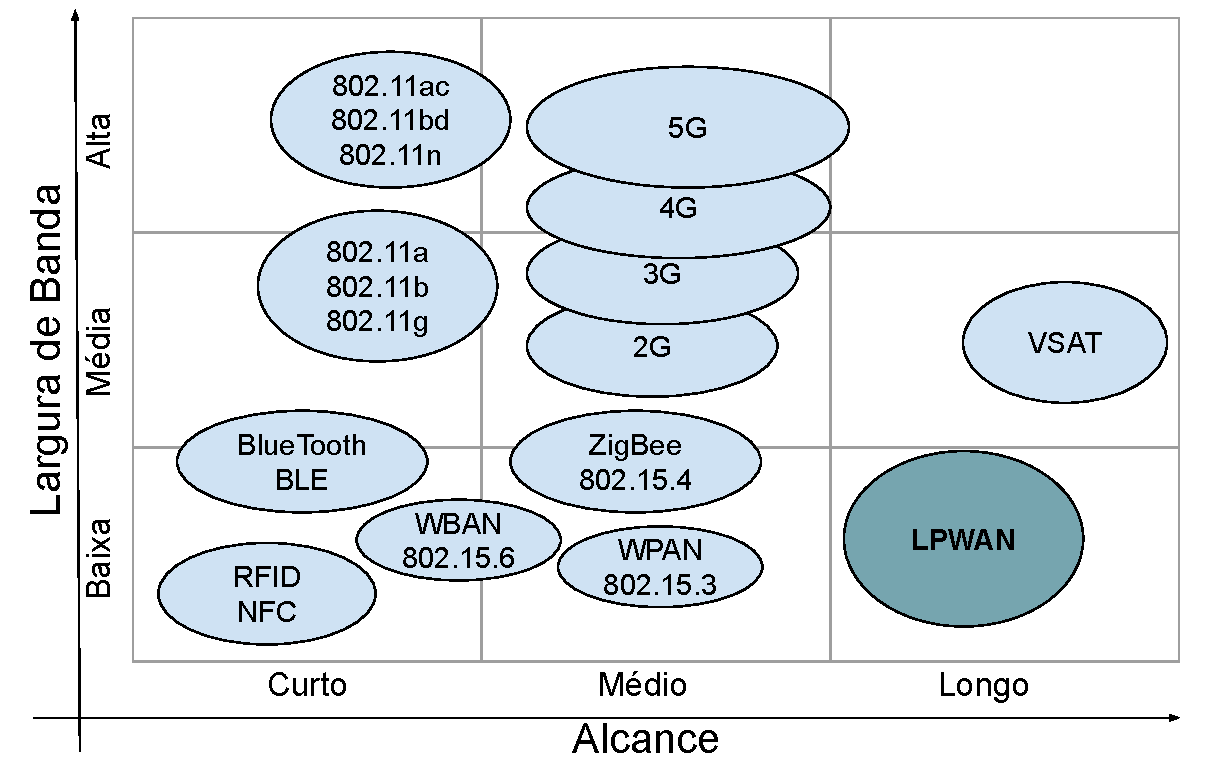
\includegraphics[scale=0.7]{img/LPWAN.pdf}
  \end{center}
  \fonte{Elaborado pelo autor.}
  \label{fig:LPWAN}
\end{figure}
%\FloatBarrier 
Redes \textit{LPWAN} tem crescido em volume devido a sua versatilidade em aplicações \textit{IoT} significativamente desde 2017. De acordo com \citeonline{Mane2021}, as duas principais tecnologias que dominam este mercado, \textit{LoRa} e \textit{Sigfox} apresentam resultados de performance compatíveis para esse tipo de aplicação, podendo ainda possuir configurações diferentes de ganhos para cada necessidade.


%%%%%%%%%%%%%%%%%%%%%%%%%%%%%%%%%%%%%%%%%%%%%%%%%%%%%%%%%%%%%%%%%%%%%%
\subsection{LoRa}
LoRa\cite{LoRaAlliance} é a camada física ou a modulação sem fio utilizada para criar o link de comunicação de longo alcance. Muitos sistemas sem fio legados usam a modulação FSK (Frequency Shifting Keying) como a camada física porque é uma modulação muito eficiente para alcançar baixa potência. O LoRa é baseado na modulação de espalhamento espectral, que mantém as mesmas características de baixa potência da modulação FSK, mas aumenta significativamente o alcance da comunicação. 

Esta comunicação é semelhante ao FM, pois modula um sinal alterando sua frequência. No entanto, enquanto um sinal FM muda a frequência instantaneamente, um sinal LoRa aumenta ou diminui a frequência lentamente ao longo de um período de tempo. Esse aumento ou diminuição gradual é chamado de \textit{chirp}, e a taxa de mudança de frequência ao longo do tempo é chamada de \textit{`chirpiness'}. 

O espalhamento espectral tem sido usado em comunicações militares e espaciais por décadas devido às longas distâncias de comunicação que podem ser alcançadas e robustez à interferência, mas o LoRa é a primeira implementação de baixo custo para uso comercial.

As redes LoRaWAN distribuem-se em uma topologia estrela, com protocolos de comunicação e acesso projetados para usar o mínimo de energia e minimizar colisões de sinal de vários terminais. Cada \textit{endpoint} envia seus dados para um \textit{gateway}, que transmite os dados para outra rede, como Ethernet ou Wi-Fi. Os dados recebidos pelo \textit{gateway} são transmitidos pela rede para um computador central que fará o armazenamento ou processamento adicional.
%%%%%%%%%%%%%%%%%%%%%%%%%%%%%%%%%%%%%%%%%%%%%%%%%%%%%%%%%%%%%%%%%%%%%%
\subsection{Sigfox}
%%%%%%%%%%%%%%%%%%%%%%%%%%%%%%%%%%%%%%%%%%%%%%%%%%%%%%%%%%%%%%%%%%%%%%

Esta abordagem única no mundo da conectividade sem fio, onde não há sobrecarga de sinalização, um protocolo compacto e otimizado e onde o compartilhamento de objetos não está conectado à rede.
A Sigfox oferece uma solução de comunicação baseada em software, onde toda a complexidade de rede e computação é gerenciada na nuvem, e não nos dispositivos. Tudo isso junto, reduz drasticamente o consumo de energia e os custos dos dispositivos conectados.


Um dos desafios mais significativos enfrentados pela Internet das Coisas (IoT) é a capacidade de adicionar nós sensores sem fio de maneira fácil e econômica. Sigfox é uma rede proprietária destinada a ouvir bilhões de objetos transmitindo dados, sem a necessidade de estabelecer e manter conexões de rede. O link sem fio precisa ser de baixa potência para que os nós possam funcionar por anos com uma única bateria e ainda ter longo alcance para que milhares de nós possam se conectar ao gateway para coletar dados.

A empresa francesa Sigfox desenvolveu um protocolo de rádio de baixa potência, implementação de rede e infraestrutura de computação em nuvem que pode ser usado para conectar milhões de dispositivos sem fio de baixa potência. Para isso, o protocolo de baixo consumo combinado com uma rede de \textit{gateways} semelhantes a sistemas de telefonia celular, mas que diferentemente de aplicações \textit{machine-to-machine} (M2M) em redes celulares, as redes Sigfox são dedicadas a dispositivos IoT para monitoramento de saúde, energia, temperatura e umidade e até mesmo sensores de segurança.

A rede foi otimizada para longo alcance e baixa potência usando modulação do tipo \textit{differential binary phase shift keying} (DBPSK). Este é um tipo de modulação robusto e altamente eficiente que transporta um bit por símbolo e não precisa de recuperação de portadora. A robustez da codificação permite o longo alcance, e a simplicidade ajuda a manter o consumo de energia baixo, pois pode ser tratado por um processador de 8 bits. Com uma taxa de dados de 100 bits/s é adequada para aplicações de nó de sensor sem fio de longo alcance e baixa potência com atualizações regulares de pequenas quantidades de dados.


%%%%%%%%%%%%%%%%%%%%%%%%%%%%%%%%%%%%%%%%%%%%%%%%%%%%%%%%%%%%%%%%%%%%%%
\subsection{Escolha do protocolo}
%%%%%%%%%%%%%%%%%%%%%%%%%%%%%%%%%%%%%%%%%%%%%%%%%%%%%%%%%%%%%%%%%%%%%%
Redes LoRaWAN e Sigfox, apresentam soluções que podem divergir sobre alguns aspectos, como o fato das redes LoRaWAN necessitarem de uma implementação da infraestrutura de rede com gateway e servidores. Já na rede Sigfox, a infraestrutura de rede é comercializada pela própria empresa, imputando à solução o pagamento de taxas relacionadas à comunicação. O quadro~\ref{qd:LoraVsSigfox} apresenta uma comparação entra as características técnicas de cada tecnologia.

\begin{quadro}
\caption{Comparação entre LoRa e Sigfox.}
\label{qd:LoraVsSigfox}
  \begin{center}
      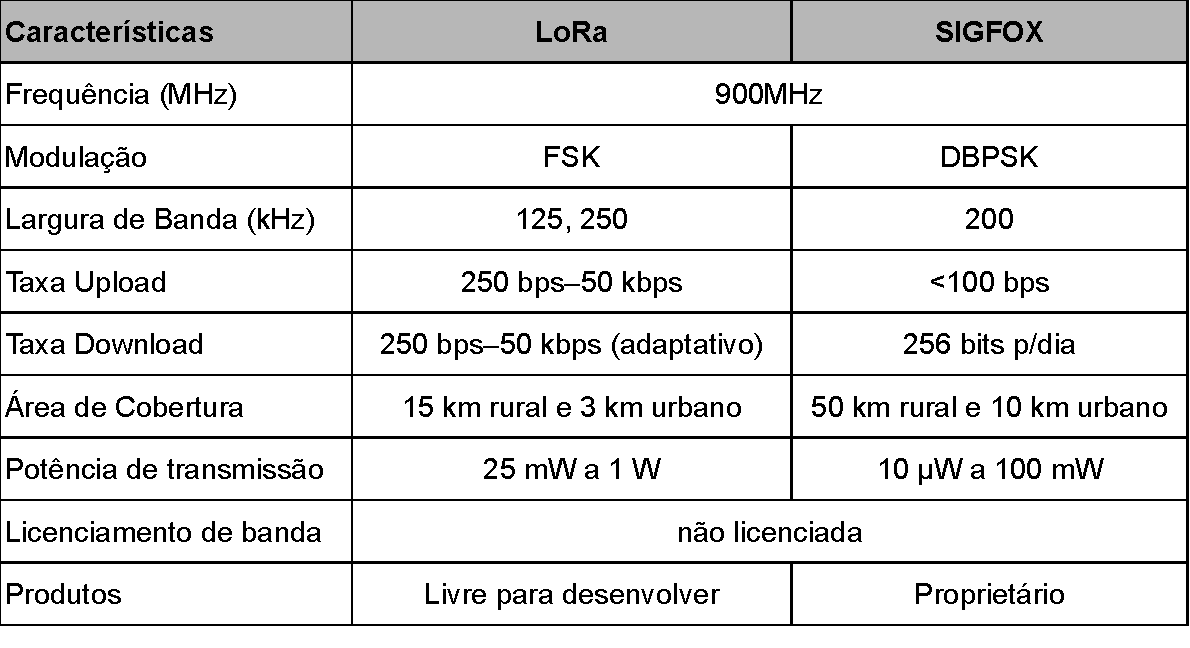
\includegraphics[scale=0.8]{img/LoraVsSigfox.pdf}
  \end{center}
\fonte{Elaborado pelo autor.}
\end{quadro}

No estudo apresentado por \citeonline{Osman2018}, concluiu-se que a tecnologia Sigfox apresenta uma menor taxa de colisões por pacote. Somando-se isso ao fato de existir uma infraestrutura de rede privada para este tipo de aplicação, pode-se dizer que a escolha deste tipo de rede apresenta vantagens.

Entretanto, cabe ressaltar que as duas tecnologias apresentam características suficientes para implementação da solução a que esse trabalho se propõe. Neste trabalho no entanto, optou-se por uso de um recurso de hardware disponibilizado pela empresa HT Micron para fins de estudo capaz de estabelecer uma comunicação do tipo indicado para redes Sigfox.
%%%%%%%%%%%%%%%%%%%%%%%%%%%%%%%%%%%%%%%%%%%%%%%%%%%%%%%%%%%%%%%%%%%%%%
\section{Energy Harvesting}
%%%%%%%%%%%%%%%%%%%%%%%%%%%%%%%%%%%%%%%%%%%%%%%%%%%%%%%%%%%%%%%%%%%%%%
\textit{Energy Harvesting} (EH) é um termo em inglês que pode ser traduzido como ``Captura de Energia'' e consiste e coletar energia de algum meio para empregar em um outro uso. Por milênios os seres humanos vêm criando e aperfeiçoando técnicas de coletar energia de um modo cada vez mais eficiente e diversificado.

As técnicas podem variar, mas pode-se coletar energia atualmente com as seguintes fontes: solar, de vibrações, térmica, cinética, piezoelétrica e de radiofrequência. Muitas fontes de energia se consolidaram no último século como a cinética em casos que transforma o movimento dos rios em energia através de usinas hidrelétrica, bem como os painéis solares que transformam a energia solar e eletricidade. Entretanto, estes meios caracterizam-se por converter grandes volumes de energia para abastecer grandes populações. 

Já em sistemas IoT que necessitam de mobilidade, esta tarefa encontra um dificultador devido ao espaço que estes capturadores de energia necessitam. Além do mais, devido a mobilidade, nem sempre algumas fontes podem estar presente, como a luz solar, uma vez que este sistema se encontre em um local fechado. 

Nestes casos, a escolha da fonte de energia deve ser analisada respeitando os critérios de disponibilidade da fonte nos locais por onde este dispositivo efetuará o seu deslocamento. Dentre as possibilidades de aproveitamento de energia para sistemas IoT, um deles se destaca por sua crescente disponibilidade. O crescente aumento do número de dispositivos de RF para redes ISM(\textit{industrial, scientific and medical}) aponta para um caminho de alta disponibilidade de potência de sinal disponível nesta banda de frequência. No Brasil, a faixa que compreende as frequências de $902MHz$ até $928MHz$ alocou-se para este tipo de aplicações. Em um estudo realizado por~\citeonline{manuel}, pode-se obter uma medição da potência de sinal de RF ao logo de uma faixa do espectro de frequências em uma estação de metrô da Inglaterra. Pode-se observar na figura~\ref{fig:espectro} que nesta mesma faixa citada acima, há uma grande alocação de potência, indicando significativa disponibilidade de energia a ser coletada.

\begin{figure}
  \caption{Densidade de potência de RF medida fora da estação Northfields London.}
  \begin{center}
      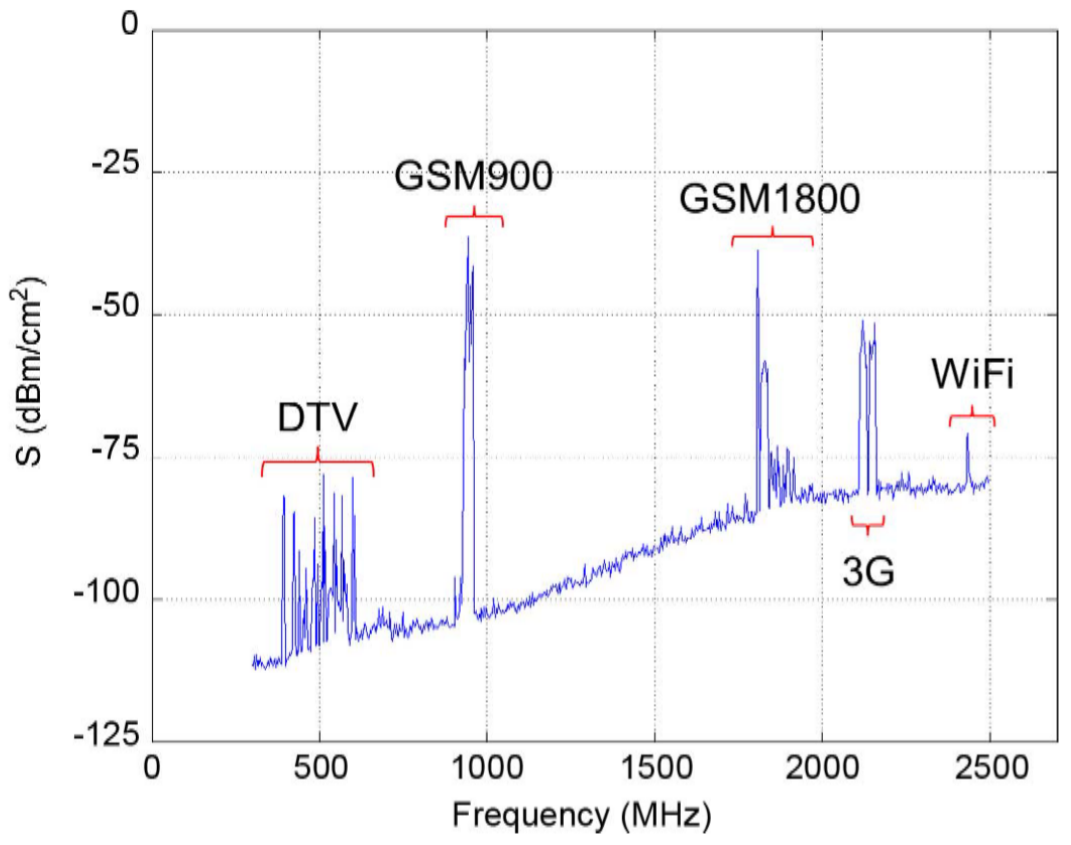
\includegraphics[scale=0.4]{img/espectro.png}
  \end{center}
  \fonte{~\cite{manuel} }
  \label{fig:espectro}
\end{figure}

%%%%%%%%%%%%%%%%%%%%%%%%%%%%%%%%%%%%%%%%%%%%%%%%%%%%%%%%%%%%%%%%%%%%%%


Todos os trabalhos mencionados no quadro~\ref{qd:correlatos} possuem as suas particularidades de aplicação à projetos que envolvem a análise ou monitoramento de redes inteligentes de distribuição de produtos perecíveis. Não necessariamente envolvendo alimentos, ou especificamente o monitoramento, mas traçando algum paralelo com o presente trabalho.
Alguns dos trabalhos são mais superficiais, outros mais profundos, porém todos demonstram alinhamento com o tema proposto.

\begin{quadro}
  \caption{Trabalhos Correlatos.}
  \begin{center}
      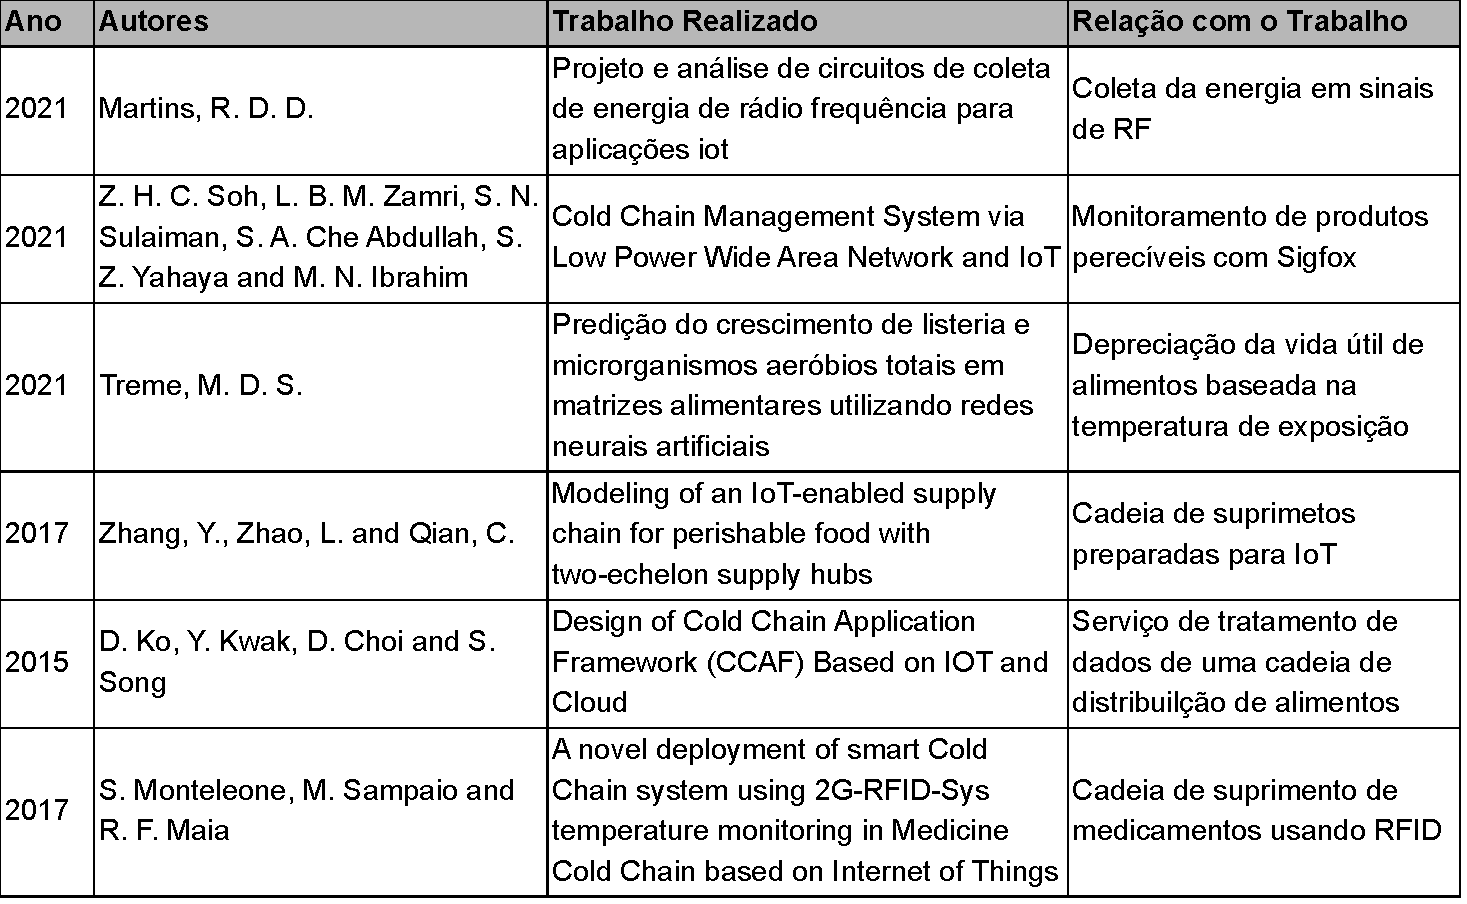
\includegraphics[scale=0.7]{img/correlatos.pdf}
  \end{center}
  \fonte{Elaborado pelo autor.}
  \label{qd:correlatos}
\end{quadro}


%%%%%%%%%%%%%%%%%%%%%%%%%%%%%%%%%%%%%%%%%%%%%%%%%%%%%%%%%%%%%%%%%%%%%%



%%%%%%%%%%%%%%%%%%%%%%%%%%%%%%%%%%%%%%%%%%%%%%%%%%%%%%%%%%%%%%%%%%%%%%
\chapter{Metodologia}
%%%%%%%%%%%%%%%%%%%%%%%%%%%%%%%%%%%%%%%%%%%%%%%%%%%%%%%%%%%%%%%%%%%%%%
A metodologia do presente trabalho é dividida em 3 principais partes. A primeira é a etapa apresenta um fluxograma de operação do sistema que ajuda a nortear a especificação das demais etapas. É na segunda etapa que ocorre a definição dos componentes de hardware que compões o dispositivo. Já na terceira etapa, são abordados as características e principais fatores que devem ser empregados no desenvolvimento do software do dispositivo.



%%%%%%%%%%%%%%%%%%%%%%%%%%%%%%%%%%%%%%%%%%%%%%%%%%%%%%%%%%%%%%%%%%%%%%
\section{Fluxograma de operação}
%%%%%%%%%%%%%%%%%%%%%%%%%%%%%%%%%%%%%%%%%%%%%%%%%%%%%%%%%%%%%%%%%%%%%%
De modo a entender as condições de operação do sistema como um todo, elaborou-se um fluxograma das suas interações. Sendo possível desta forma perceber os pontos críticos para comunicação e interfaceamento da cadeia logística em cada etapa do processo.
\begin{figure}
  \caption{Fluxograma de operação do sistema}
  \begin{center}
      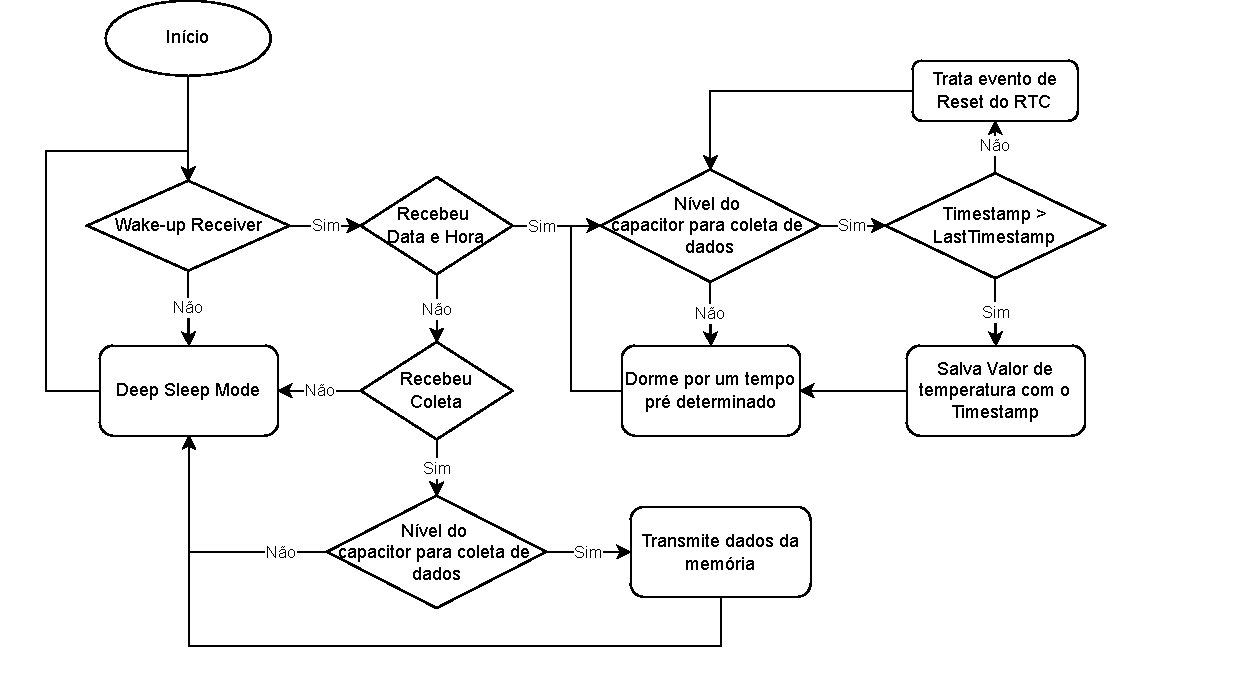
\includegraphics[scale=0.7]{img/fluxogramaOperacao.drawio.pdf}
  \end{center}
  \fonte{Elaborado pelo autor}
  \label{fig:fluxo}
\end{figure}

Um exemplo claro e notório deste tipo de avaliação se dá na inclusão de um bloco de verificação da tensão acumulada no capacitor de retensão. Com isso, se espera manter um nível mínimo de potência para manter o calendário vivo.
Na figura~\ref{fig:fluxo} pode-se ver a representação completa deste fluxo de operação.Além disso, se faz preciso a inclusão de um bloco para configuração inicial do sistema, já que informações anteriores precisam ser descartadas e isso pode ser feito simplesmente com o início de uma inserção da hora do sistema.


%%%%%%%%%%%%%%%%%%%%%%%%%%%%%%%%%%%%%%%%%%%%%%%%%%%%%%%%%%%%%%%%%%%%%%
\section{Hardware}
%%%%%%%%%%%%%%%%%%%%%%%%%%%%%%%%%%%%%%%%%%%%%%%%%%%%%%%%%%%%%%%%%%%%%%
Após a modelagem apresentada no referencial teórico, torna-se possível especificar os requisitos do dispositivo eletrônico capaz de executar as operações citadas no fluxograma de operação da figura~\ref{fig:fluxo}. Neste capítulo será detalhado cada parte do hardware proposto mostrado na figura~\ref{fig:sistema}.

\begin{figure}
  \caption{Diagrama de blocos dos componentes do hardware.}
  \begin{center}
      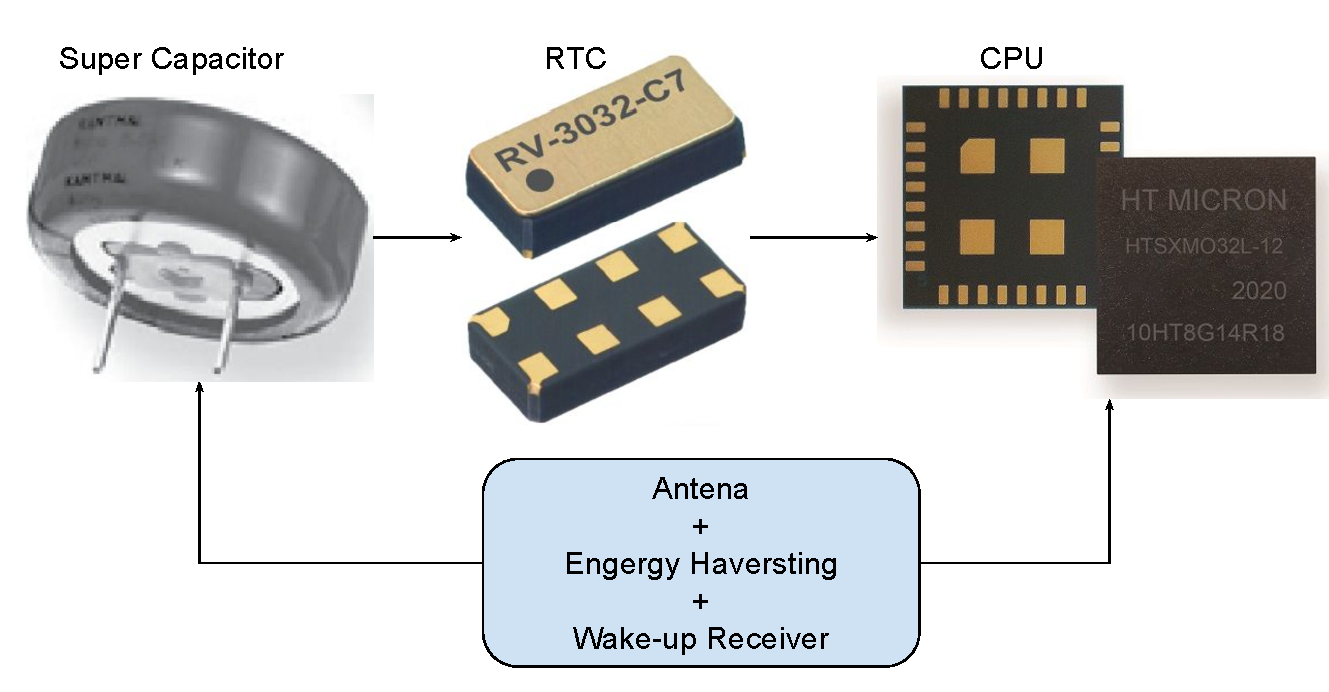
\includegraphics[scale=0.7]{img/sistema.pdf}
  \end{center}
  \fonte{Elaborado pelo autor}
  \label{fig:sistema}
\end{figure}
%%%%%%%%%%%%%%%%%%%%%%%%%%%%%%%%%%%%%%%%%%%%%%%%%%%%%%%%%%%%%%%%%%%%%%
\subsection{RTC}
%%%%%%%%%%%%%%%%%%%%%%%%%%%%%%%%%%%%%%%%%%%%%%%%%%%%%%%%%%%%%%%%%%%%%%
Aplicações de monitoramento de temperaturas em dispositivos IoT muitas vezes~\cite{Soh} podem contar com a definição de hora e data baseados no momento da transmissão, sendo dispensável a estes o uso de circuitos com \textit{Real Time Clock}(RTC), relógios de tempo real. Nos casos em que a janela de transmissão de dados ocorre um momentos distintos da coleta dos mesmos, um marcação de tempo se faz necessária para garantir a procedência desta coleta.

Para garantir essa marcação de tempo neste projeto, procurou-se obter um circuito de RTC capaz de manter sua funcionalidade por logos períodos de temo com um consumo mínimo de potência. Dentre as solução pesquisadas, cabe um destaque especial para o RV-3032~\cite{rtc} da empresa \textit{Micro Crystal} que combina um circuito integrado (CI) do tipo CMOS com um cristal ressonador interno. 

Este RTC funciona sob vácuo em embalagem cerâmica hermeticamente fechada com tampa metálica. Seu consumo de corrente em operação chega a níveis consideravelmente baixos, da ordem de nano amperes (nA). Além disso, o mesmo possuis uma compensação da precisão em função da temperatura (TXCO), que garante uma precisão de $\pm 2.5ppm$ em toda a faixa de $-40^oC$ até $85^oC$.

\begin{figure}
  \caption{Curva de operação do RV-3032}
  \begin{center}
      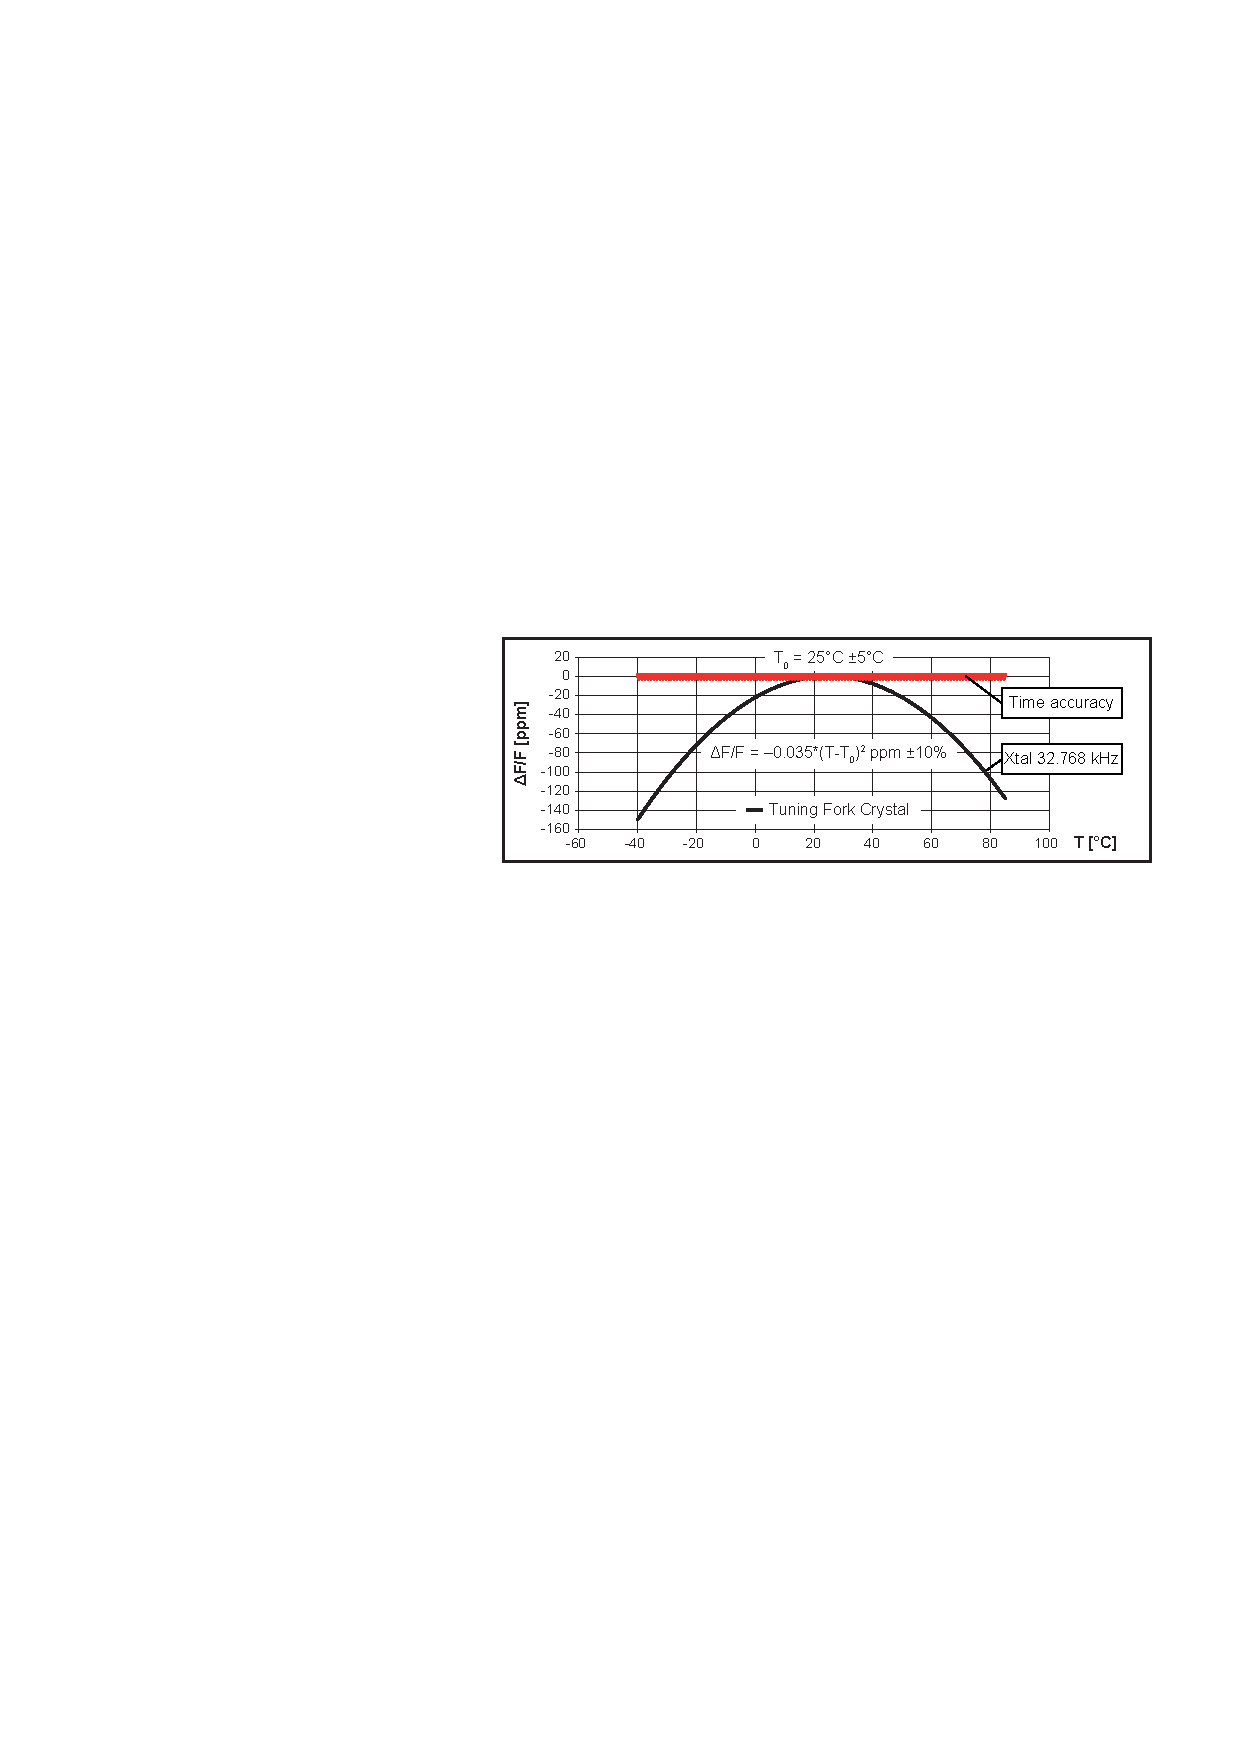
\includegraphics[scale=0.8]{img/RTCcurva.pdf}
  \end{center}
  \fonte{\citeonline{rtc}}
  \label{fig:RTC}
\end{figure}
A inserção de um sensor de temperatura e do cristal dentro do RV-3032 além de aumentar a precisão fora da temperatura convencional de $25~C$, possibilita o uso desta informação de temperatura para dispositivos IoT que possam fazer esse tipo de aquisição.
Este sensor possui uma acurácia típica de $\pm 1^oC$ que é relativamente alta, mas que não apresenta prejuízos para o estudo proposto, uma vez que a temperatura aproximada se faz suficiente para este tipo de controle.
Outra vantagem do uso deste RTC nesta aplicação, se dá em função da possibilidade de configuração de alarmes capazes de acordar o processador por uma janela de tempo pré estipulada, ou o cruzamento por uma temperatura específica. Esta função, pode ser considerada um real diferencial para a redução do consumo de operação do dispositivo, já que permite ao microcontrolador ligado ao RTC entrar em um modo profundo de economia de energia (\textit{Deep Sleep Mode}).

%%%%%%%%%%%%%%%%%%%%%%%%%%%%%%%%%%%%%%%%%%%%%%%%%%%%%%%%%%%%%%%%%%%%%%
\subsection{Super Capacitor}
%%%%%%%%%%%%%%%%%%%%%%%%%%%%%%%%%%%%%%%%%%%%%%%%%%%%%%%%%%%%%%%%%%%%%%
Dispositivos IoT podem operar de duas maneiras, conectados em algum sistema de alimentação por fios, ou alimentados para uma fonte de energia conectada somente a ele. Devido às características de mobilidade do sistema proposto neste projeto, a alimentação por algo conectado a rede elétrica não se faz possível, sendo assim necessário o uso de alguma fonte de alimentação independente.

Embora o sistema de coleta de energia dos sinais de RF estejam sempre operando, a potência capturada por este não se faz capaz de operar as funções básicas do RTC ou do microcontrolador.
Resta neste caso, recorrer a um dispositivo que armazene esta energia. Tradicionalmente, dispositivos IoT deste tipo possuem uma bateria para solucionar esta questão. Porém, baterias tendem a sofrer depreciação ao se executar cargas e descargas com uma frequência muito alta. 

Em um estudo realizado por \citeonline{supercap}, concluiu-se que o uso de super capacitores em sistemas de coleta de energia por RF pode ser uma alternativa razoável, pois embora eles possuam uma densidade de acumulo de carga centenas de vezes menores que baterias, eles se mostram eficientes em situações de carga e descarga. Neste mesmo artigo, mediu-se o tempo de carga de um capacitor e três Faraday sendo notado um tempo de cargar de aproximadamente três horas para um dispositivo comercial de conversão de energia.

Para avaliar a curva de carga e descarga do capacitor, tem-se que considerar os princípios básicos deste componente, como a relação $RC$ também chamada de constante tau ($\tau$). Na tabela~\ref{tb:capacitor} estes valores são apresentados e a partir deles, pode-se obter a curva apresentada na figura~\ref{fig:capacitor}.

% Please add the following required packages to your document preamble:
% \usepackage{booktabs}
\begin{table}
\begin{center}
\caption{Valores de $\tau$.}
\begin{tabular}{@{}cc@{}}
\toprule
\textbf{$t$}  &\textbf{ $v(t)/V_0$} \\ \midrule
$1\tau$ & $0,36788$ \\
$2\tau$ & $0,13534$ \\
$3\tau$ & $0,04979$ \\
$4\tau$ & $0,01832$ \\
$5\tau$ & $0,00674$ \\ \bottomrule
\end{tabular}
\end{center}  
\fonte{Adaptado de \citeonline{Alexander2013}}
\label{tb:capacitor}
\end{table}

\begin{figure}
  \caption{Curva de carga característica de um capacitor.}
  \begin{center}
      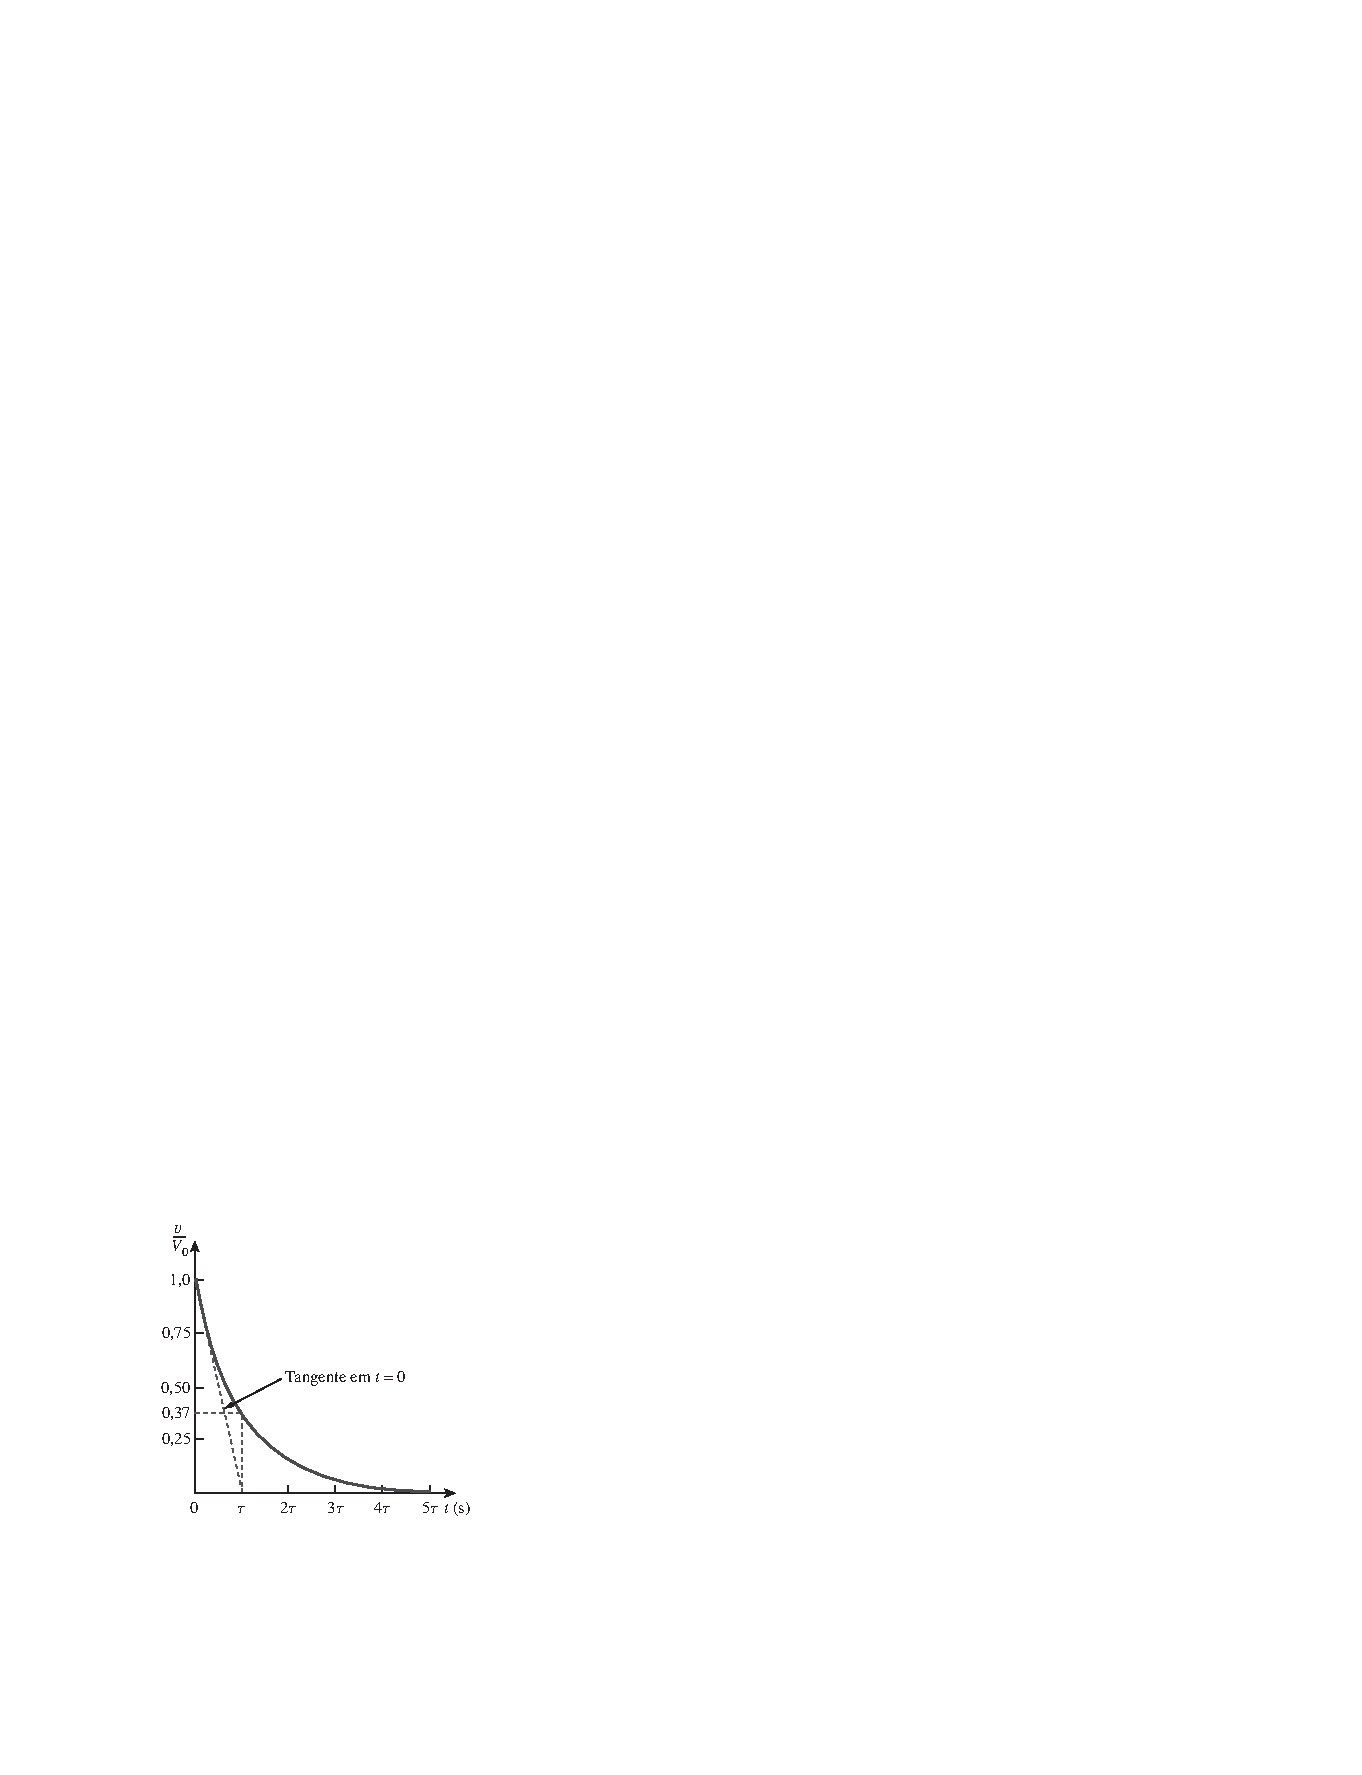
\includegraphics[scale=1]{img/capacitor.pdf}
  \end{center}
  \fonte{\citeonline{Alexander2013}}
  \label{fig:capacitor}
\end{figure}

Já para estimar o valor ideal de capacitor a ser empregado nesta solução, considerou-se a corrente máxima de $240nA$ do RTC de acordo com a informações do datasheet citado no tópico RTC. A partir disso, e considerando o range de tensão de operação ente $1,3V$ a $5$.

Com isso, obteve-se inicialmente o delta de tensão de operação através da equação\ref{eq:dv}.



\begin{equation}
    \Delta V = V_{cc}-V_{min}
  \label{eq:dv}
\end{equation}


\begin{equation}
     \Delta V =5V-1,3V = 3,7V
\end{equation}

A partir da equação do tempo de descarga, pode-se obter o valor do capacitor considerando um tempo de retensão de aproximadamente 40 dias. Estipulou-se um tempo demasiado alto para garantir longos períodos de tempo sem o recebimento de energia através do coletor. A equação~\ref{eq:T} define o cálculo do tempo e transformando na equação~\ref{eq:C} calcula-se o capacitor


\begin{equation}
    T=\frac{\Delta V \times C}{I}
  \label{eq:T}
\end{equation}


\begin{equation}
    C=\frac{(40 Dias\times 60\times60\times24) \times 240nA}{3,7V} = 224mF \cong 220mF
      \label{eq:C}
\end{equation}

Após uma busca em distribuidores de componentes, escolheu-se pelo \textit{Part Number} LM055224A~\cite{Ohmite}.


%%%%%%%%%%%%%%%%%%%%%%%%%%%%%%%%%%%%%%%%%%%%%%%%%%%%%%%%%%%%%%%%%%%%%%
\subsection{HT32SX}
%%%%%%%%%%%%%%%%%%%%%%%%%%%%%%%%%%%%%%%%%%%%%%%%%%%%%%%%%%%%%%%%%%%%%%
O iMCP–HT32SX é um circuito integrado multicomponente (MCO) projetado para fornecer uma solução de conectividade pronta para uso para aplicativos de Internet das Coisas (IoT). Ele fornece comunicações de uplink (transmissão) e downlink (recepção), e é o primeiro produto HT Micron em uma nova família de componentes sem memória. Suas pequenas dimensões, alto desempenho e baixo consumo de energia visam a melhor experiência para desenvolvedores de IoT. Possui um ARM Cortex M0+ de 32 bits (STM32L052x8) e o transceptor de baixa potência S2-LP da ST Microelectronics combinado com o SKY66420 da Skyworks Solutions que oferece todas as vantagens de desempenho, integração e conveniência da tecnologia avançada de empacotamento de semicondutores em um único chip. Este chip possui também uma EEPROM com capacidade para armazenar 2k Bytes. Na figura~\ref{fig:blockHT32SX} pode-se ver o diagrama de blocos do iMCP-HT32SX desenvolvido pela empresa HT Micron.

\begin{figure}
  \caption{Diagrama de blocos do iMCP–HT32SX.}
  \begin{center}
      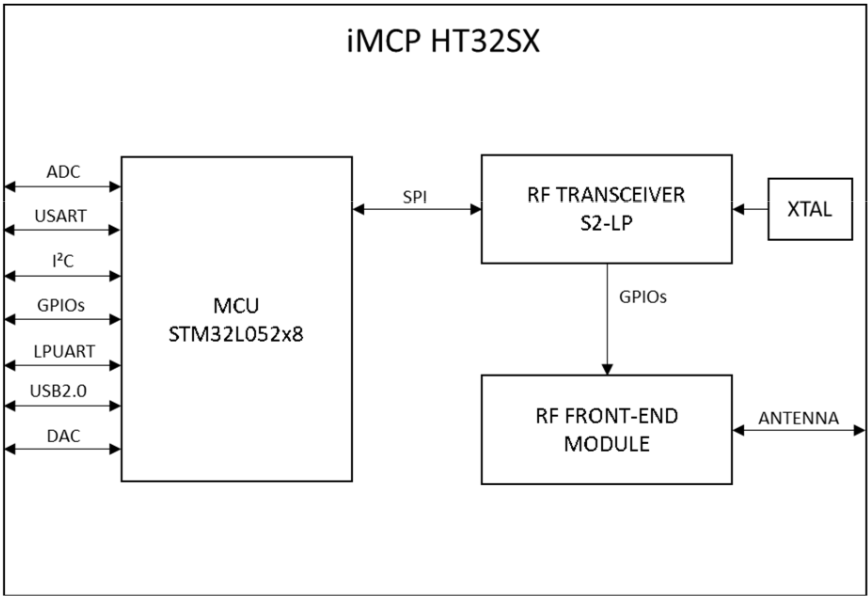
\includegraphics[scale=0.5]{img/imcpHT32sx.png}
  \end{center}
  \fonte{HT Micron\cite{Ht32sx2021} }
  \label{fig:blockHT32SX}
\end{figure}

Além dos requisitos já citados, o HT32SX ainda conta com um sensor de temperatura interno, que poderia ser utilizado para o log de eventos e assim poder-se traçar a curva desta. Porém, devido a disponibilidade de um sensor de temperatura dentro do RTC, optou-se por utilizar este e assim evitar a retirada do modo profundo de economia de energia do microcontrolador para executar esta tarefa.
%%%%%%%%%%%%%%%%%%%%%%%%%%%%%%%%%%%%%%%%%%%%%%%%%%%%%%%%%%%%%%%%%%%%%%
\subsection{HTSXMO32L-22}
%%%%%%%%%%%%%%%%%%%%%%%%%%%%%%%%%%%%%%%%%%%%%%%%%%%%%%%%%%%%%%%%%%%%%%
A Placa de Avaliação iMCP HTSXMO32L-22 foi projetada para ser uma plataforma de desenvolvimento e facilitar o primeiro contato de novos usuários com o iMCP HT32SX, além de fornecer ao usuário avançado para começar a programar e desenvolver produtos imediatamente com estrutura mínima. Todos os recursos do HT32SX estão disponíveis na placa de avaliação. Duas opções de alimentação podem ser usadas: conexão USB ou bateria externa. A placa de avaliação mudará automaticamente para alimentação USB quando estiver disponível. A bateria externa torna a placa de avaliação portátil, tornando fácil testar a conectividade do Sigfox em qualquer lugar que você vá. Na figura~\ref{fig:placaHT32SX} pode-se ver a Placa iMCP HTSXMO32L-22 desenvolvida pela empresa HT Micron.

\begin{figure}
  \caption{Placa iMCP HTSXMO32L-22.}
  \begin{center}
      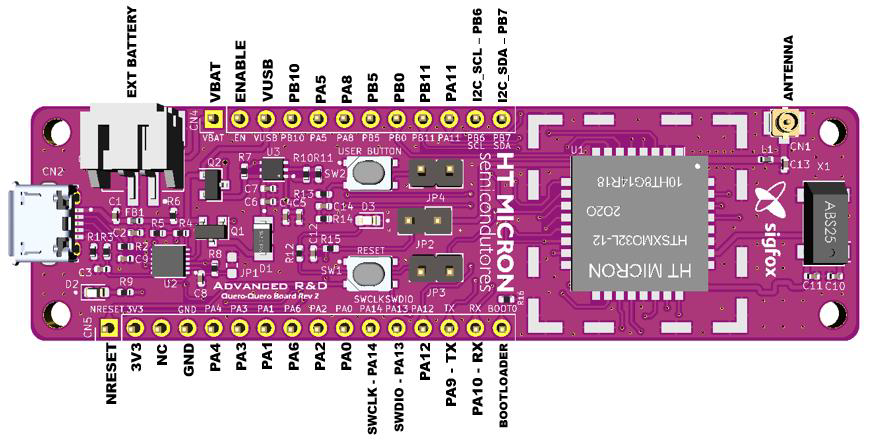
\includegraphics[scale=0.5]{img/placa.png}
  \end{center}
  \fonte{HT Micron\cite{HTSXMO32L} }
  \label{fig:placaHT32SX}
\end{figure}

%%%%%%%%%%%%%%%%%%%%%%%%%%%%%%%%%%%%%%%%%%%%%%%%%%%%%%%%%%%%%%%%%%%%%%
\subsection{Wake-up Receiver}
%%%%%%%%%%%%%%%%%%%%%%%%%%%%%%%%%%%%%%%%%%%%%%%%%%%%%%%%%%%%%%%%%%%%%%
Devido a escolha por um sistema sem baterias, algumas contensões precisam ser executadas para a operação do sistema de forma a desperdiçar o mínimo de energia. Embora o monitoramento de temperaturas de operação implique em um custo energético, o mesmo em nada se compara a uma transmissão de rádio, ou até mesmo a manutenção de uma recepção de rádio por longos períodos de tempo. Por isso se faz necessário um mecanismo responsável por ligar o receptor para aguardar uma comunicação. Neste cenário, o custo energético se mantém apenas por um intervalo curto de tempo. Mas para identificar o início dessa comunicação, utiliza-se o método chamada \textit{Wake-up Receive}. 

Com base nisso, \citeonline{ferreira} classifica como vantajosa a utilização de um circuito receptor adicional de baixa potência operando como um gatilho para o receptor principal. Com a identificação deste sinal, um microcontrolador pode ser acordado por interrupção e executar a inicialização do receptor principal.

Uma vez que o sistema esteja acordado, ele pode inclusive realizar uma medição da energia armazenada no sistema de coleta para decidir pelo ligamento do receptor ou não. Uma vez que o sistema identifique as condições propícias para para o receptor de rádio principal, este pode aguardar pelos comandos básicos e após um tempo o sistema volta a dormir em modo profundo de consumo de energia.
%%%%%%%%%%%%%%%%%%%%%%%%%%%%%%%%%%%%%%%%%%%%%%%%%%%%%%%%%%%%%%%%%%%%%%
\section{\textit{Software}}
%%%%%%%%%%%%%%%%%%%%%%%%%%%%%%%%%%%%%%%%%%%%%%%%%%%%%%%%%%%%%%%%%%%%%%
Após a modelagem, deve-se implementar o modelo de software baseado nos levantamentos do fluxograma de operação mostrado na figura~\ref{fig:fluxo}. A partir da documentação e bibliotecas de exemplo contido no repositório do fabricante do módulo HTSXMO32L-22, tornou-se possível escolher entre os modelos uma solução adequada para este projeto.
Dentre as soluções oferecidas, selecionou-se a \textit{P2P Demo Application} devido a sua simplicidade de operação e possibilidade de adaptação para as necessidades do projeto. Na figura~\ref{fig:p2p} pode-se ver o diagrama da maquina de estados finita do exemplo selecionado.

\begin{figure}
  \caption{Diagrama da máquina de estados finita.}
  \begin{center}
      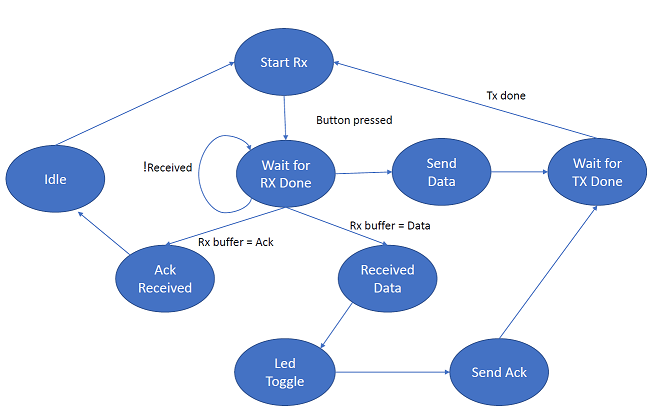
\includegraphics[scale=0.8]{img/p2p_fsm.PNG}
  \end{center}
  \fonte{HT Micron\cite{HTSXMO32L} }
  \label{fig:p2p}
\end{figure}

Este algorítimo basicamente mantém o seu rádio receptor sempre ativo e é capaz de ligar o transmissor a qualquer momento a partir de um evento de botão. Dentre as alterações necessárias para operação de acordo com este trabalho, destaca-se a alteração da funcionalidade do botão para simular eventos do sistema de \textit{Wake-up Receiver}. Desta forma, pode-se medir tanto a quantidade de energia dos seguintes estados de operação:
\begin{itemize}
    \item Modo profundo de economia de energia
    \item Consumo do receptor ligado por segundo
    \item Consumo durante a transmissão de dados
    \item Consumo para escrita na memória
    \item Consumo para conversa com o RTC
\end{itemize}

Sequencialmente pode-se definir um protocolo de comunicação para estabelecer os dois comandos descritos no fluxograma de operação para inicializar uma nova medição e para coletar os dados armazenados durante o processo de transporte.

Alternativamente, pode-se reduzir o a potência do rádio para obter melhores resultados em termos de economia de energia, já que o uso da rede Sigfox não se faz necessária para envio de dados e sim o uso de um dispositivo projetado especificamente para coleta e inicio de operação.

%%%%%%%%%%%%%%%%%%%%%%%%%%%%%%%%%%%%%%%%%%%%%%%%%%%%%%%%%%%%%%%%%%%%%%

\chapter{Cronograma}

\begin{enumerate}
	\item \label{escolhatema} Estudo e escolha do tema.
	\item \label{refteorico} Fundamentação teórica.
	\item \label{metodologia} Estudo metodológico.
	\item \label{esctcci} Escrita do TCC I.
	\item \label{comunica} Estrutura da comunicação.
	\item \label{fonte} Dimensionamento da fonte.
	\item \label{captacao} Captação de energia
	\item \label{exibicao} Sistema de exibição de dados 
	\item \label{integracaomec} Integração do mecânica do coletor com o rádio.
	\item \label{devapp} Desenvolvimento da camada de integração.
	\item \label{integracaosistema} Integração de todos os módulos que compõe o sistema.
	\item \label{testc} Testes e correções.
	\item \label{comapracoes} Comparar desempenho entre os diferentes tipos de protocolo.
	\item \label{esctccii} Escrita do TCC II.
\end{enumerate}

\definecolor{midgray}{gray}{.5}
\begin{table}[!htbp]
	\centering
		\begin{tabular}{|c|c|c|c|c|c|c|c|c|c|c|}
		\hline
		&\multicolumn{9}{c|}{2022}\\
		\hline
		Fev.&Mar.&Abr.&Mai.&Jun.&Jul.&Ago.&Set.&Out.&Nov.\\
		\hline
		\ref{escolhatema}&\cellcolor{midgray}&&&&&&&&\\
		\hline
		\ref{refteorico}&&\cellcolor{midgray}&\cellcolor{midgray}&\cellcolor{midgray}&&&&&\\
		\hline
		\ref{metodologia}&&&\cellcolor{midgray}&\cellcolor{midgray}&&&&&\\
		\hline
		\ref{esctcci}&&\cellcolor{midgray}&\cellcolor{midgray}&\cellcolor{midgray}&&&&&\\
		\hline
		\ref{comunica}&&&&&\cellcolor{midgray}&&&&\\
		\hline
		\ref{fonte}&&&&&\cellcolor{midgray}&\cellcolor{midgray}&&&\\
		\hline	
		\ref{captacao}&&&&&&\cellcolor{midgray}&&&\\
		\hline
		\ref{exibicao}&&&&&&\cellcolor{midgray}&\cellcolor{midgray}&\cellcolor{midgray}&\\
		\hline
		\ref{integracaomec}&&&&&&&\cellcolor{midgray}&\cellcolor{midgray}&\\
		\hline
		\ref{devapp}&&&&&&&&\cellcolor{midgray}&\\
		\hline	
		\ref{integracaosistema}&&&&&&&&\cellcolor{midgray}&\\
		\hline	
		\ref{testc}&&&&&&&&\cellcolor{midgray}&\\
		\hline	
		\ref{comapracoes}&&&&&&&\cellcolor{midgray}&\cellcolor{midgray}&\cellcolor{midgray}\\
		\hline
		\ref{esctccii}&&&&&&&\cellcolor{midgray}&\cellcolor{midgray}&\cellcolor{midgray}\\
		\hline		
		\end{tabular}
\end{table}
% Adicionar demais capítulos aqui

% ----------------------------------------------------------
% ELEMENTOS PÓS-TEXTUAIS
% ----------------------------------------------------------
\postextual
% ----------------------------------------------------------

% ----------------------------------------------------------
% Referências bibliográficas
% ----------------------------------------------------------
\bibliography{referencias} % caminho para o arquivo bib


%% ----------------------------------------------------------
% Apêndices
% ----------------------------------------------------------
\pdfstringdefDisableCommands{\let\uppercase\relax}
% ---
% Inicia os apêndices
% ---
\begin{apendicesenv}

% Imprime uma página indicando o início dos apêndices
\partapendices

% ----------------------------------------------------------
\chapter{Quisque libero justo}
% ----------------------------------------------------------

\lipsum[50]

% ----------------------------------------------------------
\chapter{Nullam elementum urna vel imperdiet sodales elit ipsum pharetra ligula
ac pretium ante justo a nulla curabitur tristique arcu eu metus}
% ----------------------------------------------------------
\lipsum[55-57]

\end{apendicesenv}
% --- % Adiciona os apêndices


% ----------------------------------------------------------
% Anexos
% ----------------------------------------------------------

% ---
% Inicia os anexos
% ---
\begin{anexosenv}

% Imprime uma página indicando o início dos anexos
\partanexos


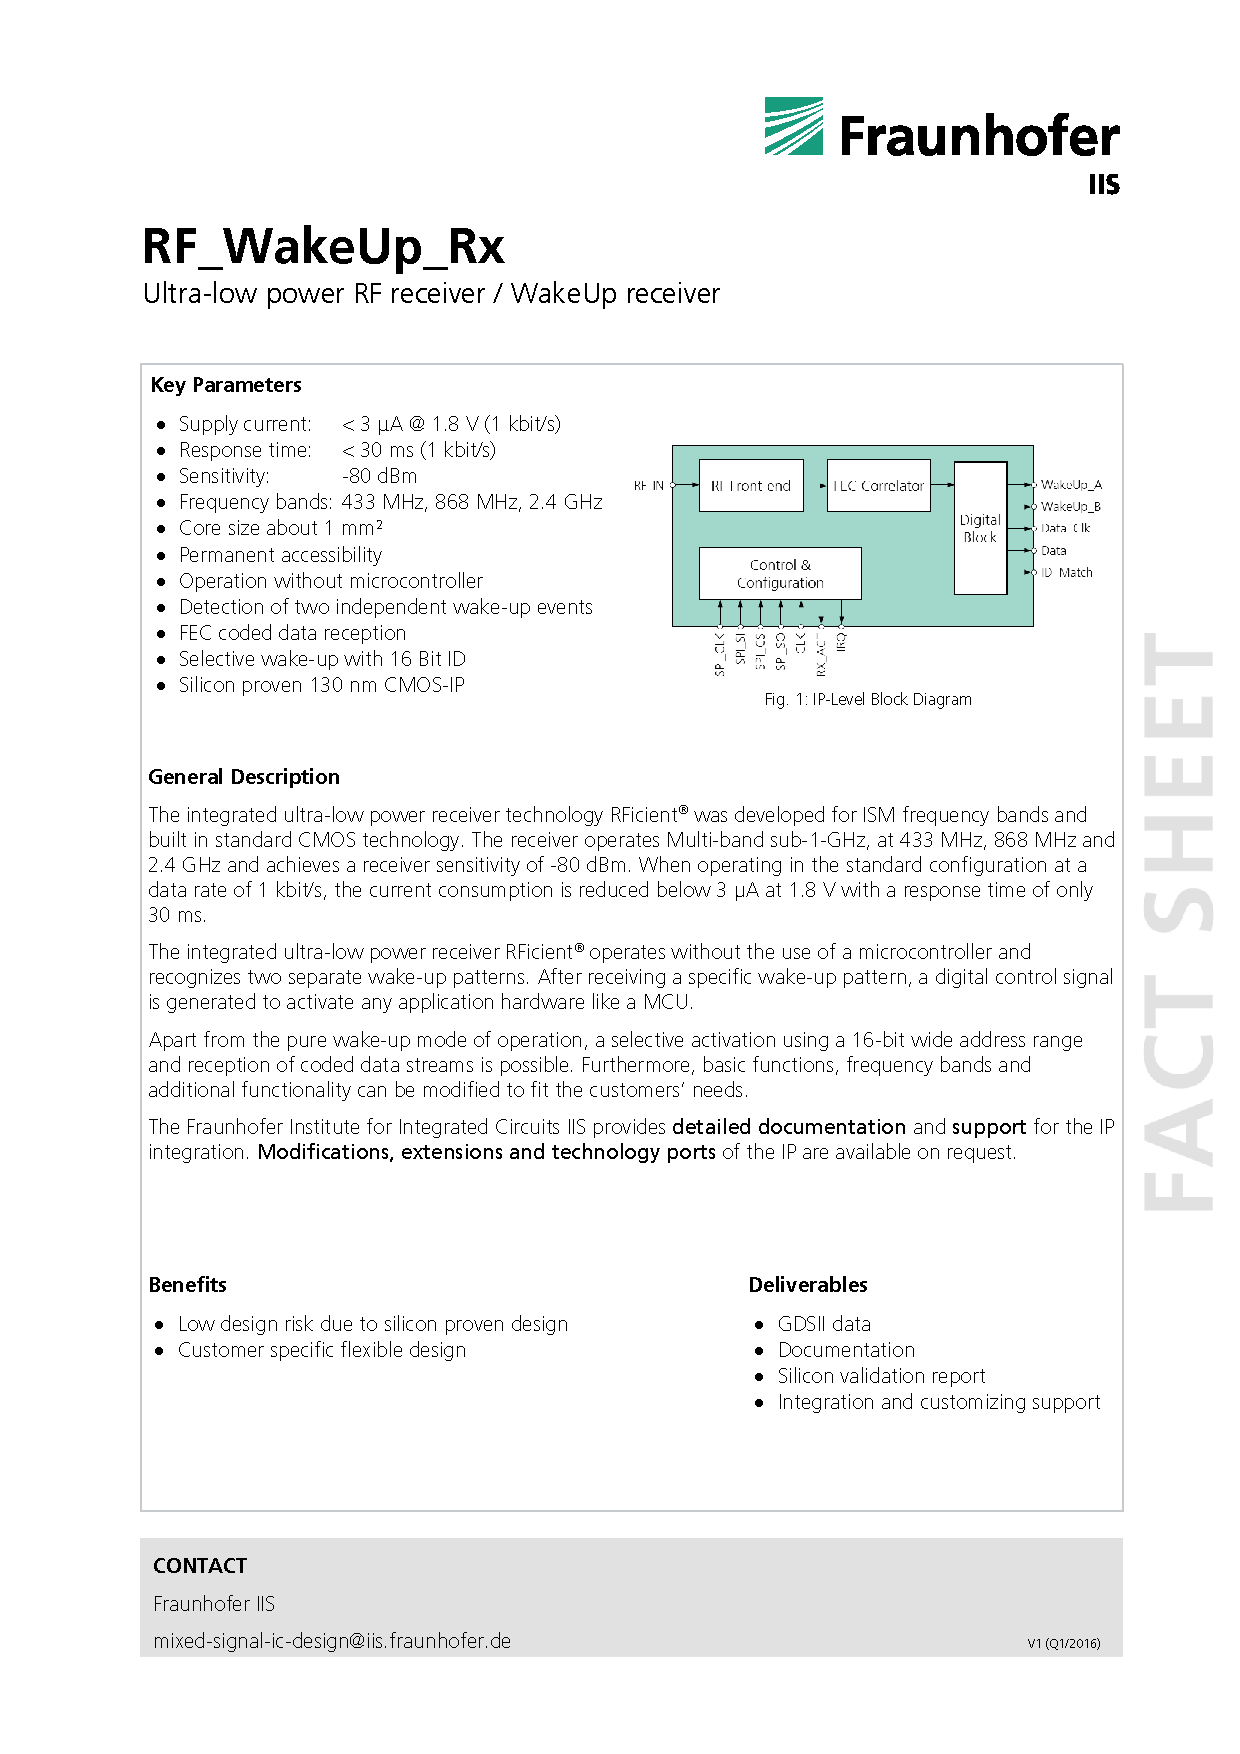
\includepdf[
    scale=0.87,
    pages=-,
    pagecommand=\chapter{Folha de dados do chip de \textit{wake-up receiver}.}\label{ax:wake}
    ]{Anexo/Factsheet-WakeUp.pdf}


\end{anexosenv} % Adiciona os anexos

%---------------------------------------------------------------------
% INDICE REMISSIVO
%---------------------------------------------------------------------
%\phantompart
%\printindex
%---------------------------------------------------------------------

\end{document}
